\chapter{The Gaussian Integers}
\label{chapter:gaussian-integers}

\section{Definition and Basic Properties of the Gaussian Integers}

\begin{figure}[t]
  \centering
  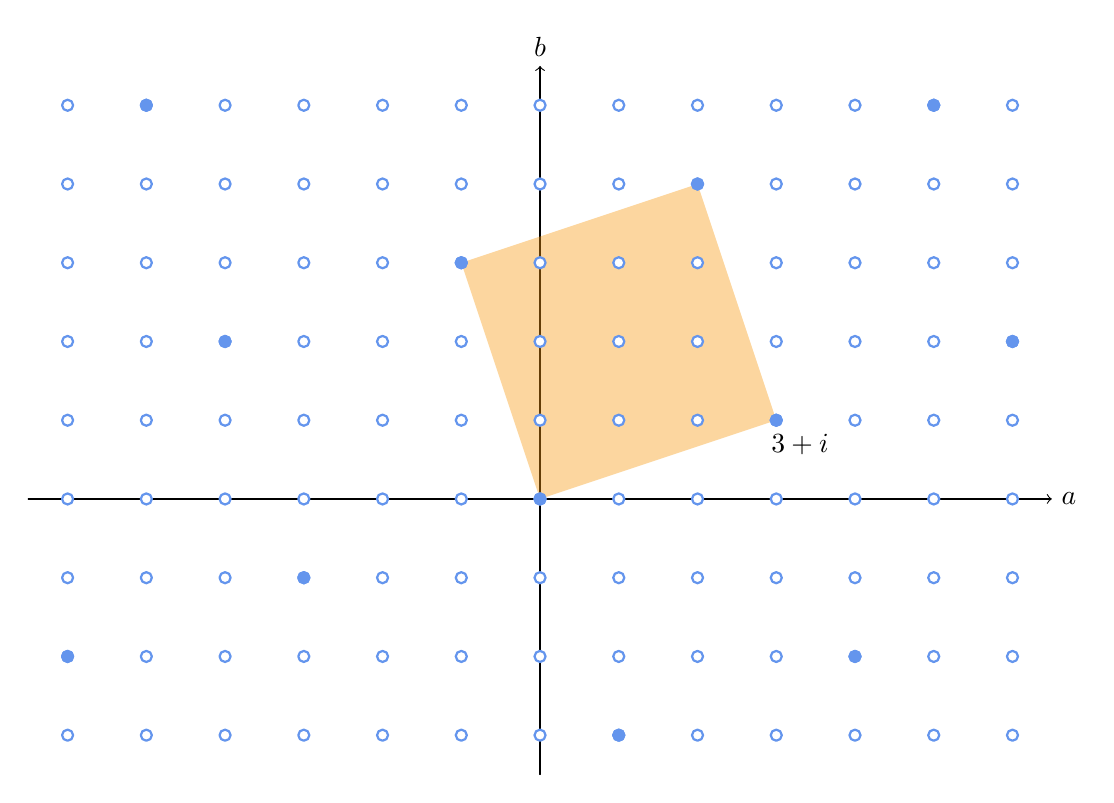
\begin{tikzpicture}[scale=1,line join=round,line cap=round]
    
    \draw[->] (-6.5,0) -- (6.5,0) node[right] {$a$};
    \draw[->] (0,-3.5) -- (0,5.5) node[above] {$b$};

    \fill[YellowOrange,opacity=.4] (0,0) -- (3,1) -- (2,4) -- (-1,3) -- cycle;

    \foreach \x in {-6,-5,-4,-3,-2,-1,0,1,2,3,4,5,6} {
      \foreach \y in {-3,-2,-1,0,1,2,3,4,5} {
        \draw[CornflowerBlue,fill=white,thick] (\x,\y) circle (2pt);
      }
    }

    \draw[CornflowerBlue,fill=CornflowerBlue,thick] (-6,-2) circle (2pt);
    \draw[CornflowerBlue,fill=CornflowerBlue,thick] (-3,-1) circle (2pt);
    \draw[CornflowerBlue,fill=CornflowerBlue,thick] (0,0) circle (2pt);
    \draw[CornflowerBlue,fill=CornflowerBlue,thick] (3,1) circle (2pt);
    \node[xshift=2ex,yshift=-2ex] at (3,1) {$3+i$};
    \draw[CornflowerBlue,fill=CornflowerBlue,thick] (6,2) circle (2pt);
    \draw[CornflowerBlue,fill=CornflowerBlue,thick] (-4,2) circle (2pt);
    \draw[CornflowerBlue,fill=CornflowerBlue,thick] (-1,3) circle (2pt);
    \draw[CornflowerBlue,fill=CornflowerBlue,thick] (2,4) circle (2pt);
    \draw[CornflowerBlue,fill=CornflowerBlue,thick] (5,5) circle (2pt);
    \draw[CornflowerBlue,fill=CornflowerBlue,thick] (4,-2) circle (2pt);
    \draw[CornflowerBlue,fill=CornflowerBlue,thick] (1,-3) circle (2pt);
    \draw[CornflowerBlue,fill=CornflowerBlue,thick] (-5,5) circle (2pt);
  \end{tikzpicture}
  \caption[The Gaussian integers]{\label{figure:gaussian-integers}The set of Gaussian integers. All the multiples of $3+i$ are marked with solid dots, and all the nonmultiples are marked with open dots. The norm of $3+i$ is the area of the square shaded in orange.}
\end{figure}

\begin{definition}
  A \define{Gaussian integer} is an expression of the form
  \begin{equation*}
    a+bi
  \end{equation*}
  in which $a$ and $b$ are integers. We say that the \define{real part} of $a+bi$ is the integer $a$, and the \define{complex part} of $a+bi$ is the integer $b$.

  We will write $\mathbb{Z}[i]$ for the set of Gaussian integers. Gaussian integers are added, subtracted, and multiplied according to the following rules:
  \begin{align*}
    (a+ib)+(c+id) & = (a+c)+i(b+d) \\
    (a+ib)-(c+id) & = (a-c)+i(b-d) \\
    (a+ib)(c+id)  & = (ac-bd)+i(ad+bc).
  \end{align*}
\end{definition}

\begin{definition}
  The \define{norm} of a Gaussian integer $\alpha=a+bi$ is given by
  \begin{equation*}
    N(\alpha)=a^2+b^2.
  \end{equation*}
\end{definition}

\begin{proposition}[The Brahmagupta--Fibonacci identity]
  The norm function $N$ is completely multiplicative in the sense that
  \begin{equation*}
    N(\alpha\beta)=N(\alpha)N(\beta)
  \end{equation*}
  for any two Gaussian integers $\alpha$ and $\beta$.
\end{proposition}

\begin{definition}
  A Gaussian integer $\alpha$ is said to \define{divide} a Gaussian integer $\beta$ if there exists a Gaussian integer $\kappa$ such that
  \begin{equation*}
    \kappa\alpha=\beta.
  \end{equation*}
  Any Gaussian integer dividing $1$ is called a \define{unit}.
\end{definition}

\begin{theorem}
  The only units among the Gaussian integers are $\pm 1$ and $\pm i$.
\end{theorem}

\section{Euclidean Division of Gaussian Integers}

\begin{example}
  The following choices of $\alpha$ and $\beta$ show that there can be multiple pairs of Gaussian integers $\kappa$ and $\rho$ with $N(\rho)<N(\beta)$ such that
  \begin{equation*}
    \alpha=\kappa\beta+\rho.
  \end{equation*}
  \begin{enumerate}
  \item Consider $\alpha := 8+11i$ and $\beta=3+i$, so that $N(\beta)=10$. Then
    \begin{equation*}
      \frac{\alpha}{\beta}=\frac{(8+11i)(3-i)}{3^2+1^2}=\frac{35+25i}{10}=(3+2i)+\frac{1+i}{2}.
    \end{equation*}
    This shows that $\alpha = (3+2i)\beta + (1+2i)$. Note that $N(1+2i)=5<10$. However, we can also write
    \begin{align*}
      \alpha & = (4+2i)\beta + (-2+i), & N(-2+i) & = 5,\\
      \alpha & = (3+3i)\beta + (2-i), & N(2-i) & = 5, \\
      \alpha & = (4+3i)\beta + (-2-i), & N(-2-i) & = 5.
    \end{align*}
  \item Consider $\alpha := 2+3i$ and $\beta=4$, so that $N(\beta)=16$. Then we can write
    \begin{align*}
      \alpha & = i\beta + (2-i), & N(2-i) & = 5, \\
      \alpha & = (1+i)\beta + (-2-i), & N(-2-i) & = 5.
    \end{align*}
  \end{enumerate}
\end{example}

Define the half-open fundamental square to be the following subset of $\mathbb{C}$:
\begin{equation*}
  \mathcal{S}:=\big\{x+yi\in\mathbb{C}\mid -\tfrac{1}{2}<x,y\leq \tfrac{1}{2}\big\}.
\end{equation*}

\begin{theorem}
  Consider two Gaussian integers $\alpha$ and $\beta$ with $N(\alpha)>N(\beta)$. Then there exist unique Gaussian integers $\kappa$ and $\rho$ with $N(\rho)<N(\beta)$, such that
  \begin{equation*}
    \alpha=\kappa\beta+\rho
  \end{equation*}
  and $\frac{\rho}{\beta}\in\mathcal{S}$.
\end{theorem}

\section{The Greatest Common Divisor of Gaussian Integers}

The definition of a greatest common divisor carries over directly from the integers to the Gaussian integers.

\begin{definition}
  Consider two Gaussian integers $\alpha$ and $\beta$. A Gaussian integer $\delta$ is said to be the \define{greatest common divisor} of $\alpha$ and $\beta$ if it satisfies the following logical equivalence for every Gaussian integer $\xi$:
  \begin{equation*}
    (\xi\mid \alpha)\land (\xi\mid\beta) \Leftrightarrow (\xi\mid\delta).
  \end{equation*}
\end{definition}

\section{Primes in the Gaussian Integers}

\section{Fermat's Two-Square Theorem}

\section{The Biquadratic Character of \texorpdfstring{$-1$}{-1}}

\exercises

\begin{challenge}
  \exercise
  \begin{subexenum}
  \item Consider a Gaussian integer $\alpha=a+bi$ such that $\gcd(a,b)=1$. Show that the number of Gaussian integers in the interior (that is, not on the boundary) of the square spanned by the Gaussian integers $0$, $\alpha$, $i\alpha$, and $(1+i)\alpha$ is $N(\alpha)-1$. See \zcref{figure:gaussian-integers} for such a square with $\alpha=3+i$.
  \item For any Gaussian integer $\alpha=a+bi$, determine the number of Gaussian integers in the interior of the square spanned by the Gaussian integers $0$, $\alpha$, $i\alpha$, and $(1+i)\alpha$.
    % # Interior points = N(\alpha) - 2\gcd(|a|,|b|) + 1.
  \end{subexenum}
\end{challenge}

%%% Local Variables:
%%% mode: latex
%%% TeX-master: "elementary-number-theory"
%%% TeX-engine: luatex
%%% End:
